\documentclass{beamer}

%\usetheme[framenumber,totalframenumber]{UniversiteitGent}
%\usetheme[faculty=di,framenumber,totalframenumber]{UniversiteitGent}
%\usetheme[faculty=we,usecolors,framenumber,totalframenumber]{UniversiteitGent}
%\usetheme[language=english,framenumber,totalframenumber]{AlleghenyCollege}
\usetheme{AnnArbor}
\usecolortheme{dove}

\title{CMPSC 390 \\ Crypto Fundamentals }
\author{Janyl Jumadinova \\ $ $ \\ Credit: Authors of ``Bitcoin and Cryptocurrency Technologies"}
\date{January 21-22, 2021}

\long\def\omitit#1{}

\usepackage{hyperref}

\begin{document}

\begin{frame}
  \titlepage
\end{frame}

%%%%%%%%%%%% Slide %%%%%%%%%%%%%%%%%%%%%%%%%%%%%%%%%%%%%%%%%%%%%%%%%%%
\begin{frame}
  \frametitle{Cryptocurrency Components}
	\begin{itemize}
		\item \textcolor{brown}{Identity}:  an account (\textcolor{brown}{node}) in the system.
		\item \textcolor{brown}{Transactions:} sending and receiving  units of cryptocurrency.
		\item \textcolor{brown}{Distributed Ledger:} a public record of transaction history (blockchain).
		\item \textcolor{brown}{Trustless Consensus:} agreement on changes to the ledger.
	\end{itemize}
\end{frame}
%%%%%%%%%%%% Slide %%%%%%%%%%%%%%%%%%%%%%%%%%%%%%%%%%%%%%%%%%%%%%%%%%%
\begin{frame}
  \frametitle{Cryptographic Hash Functions}
  
	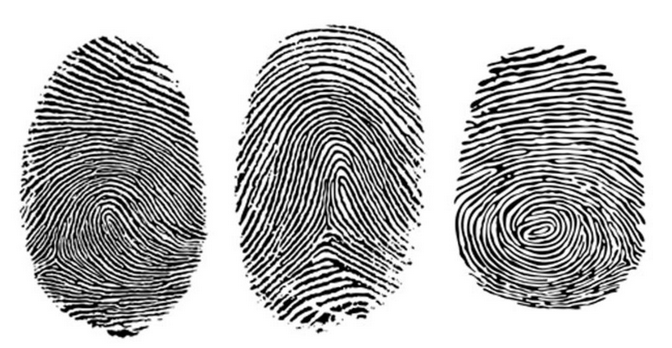
\includegraphics[scale=0.3]{fingers}
	\begin{itemize}
		\item \textcolor{brown}{Cryptographic Hash Functions}:  ensure trust in communication in a trustless system. \pause
		\item Input of any size, fixed-size output (e.g., 256 bits).
	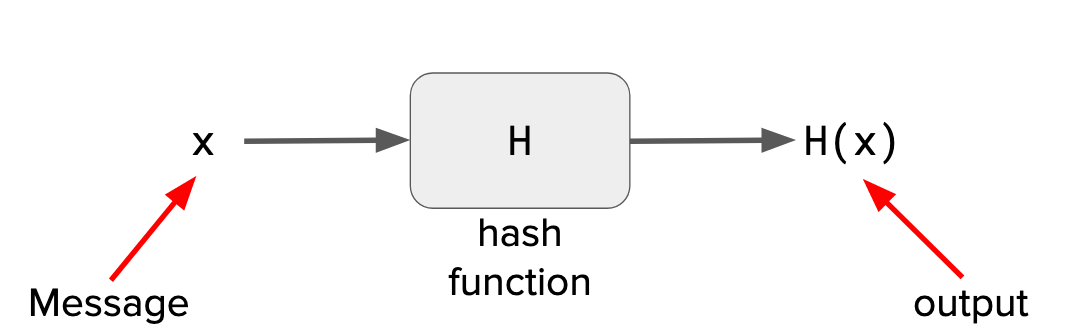
\includegraphics[scale=0.5]{hash}
	\end{itemize}
\end{frame}
%%%%%%%%%%%% Slide %%%%%%%%%%%%%%%%%%%%%%%%%%%%%%%%%%%%%%%%%%%%%%%%%%%
\begin{frame}
  \frametitle{Security Properties}
  
  \begin{block}{\textbf{Hash property 1:}}
  \textcolor{brown}{\textbf{Collision resistance}} \\
Nobody can find $x$ and $y$ such that $x != y$ and $H(x)=H(y)$.
 	\end{block}
	\centering
	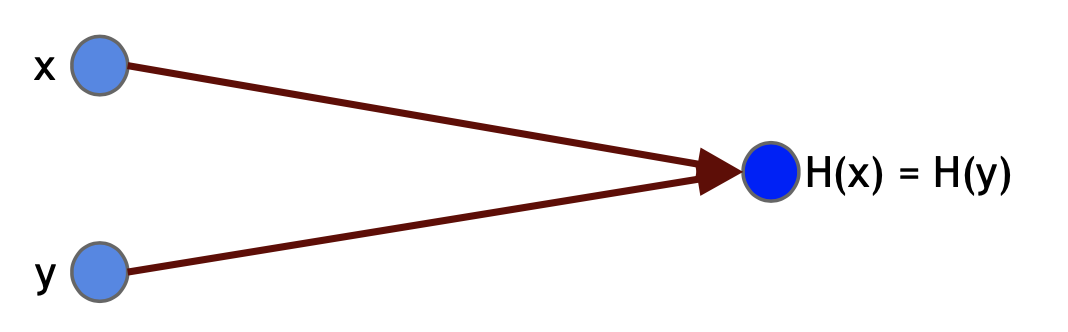
\includegraphics[scale=0.5]{property1}  \\ 
	Nobody can find this!
\end{frame}
%%%%%%%%%%%% Slide %%%%%%%%%%%%%%%%%%%%%%%%%%%%%%%%%%%%%%%%%%%%%%%%%%%
\begin{frame}
  \frametitle{Collisions}
  Collisions exist ... \pause but can anyone find them?
	\begin{itemize}
		\item Try $2^{130}$ randomly chosen inputs.
		\item There is $99.8\%$ chance that two of them will collide. \pause 
		\item This works no matter what $H$ is ... \pause but it takes too long to matter.
		\pause
		\item No $H$ has been \textbf{proven} collision-free.
	\end{itemize}

\end{frame}
%%%%%%%%%%%% Slide %%%%%%%%%%%%%%%%%%%%%%%%%%%%%%%%%%%%%%%%%%%%%%%%%%%
\begin{frame}
  \frametitle{Security Properties}
  
  \begin{block}{\textbf{Hash property 2}:}
  \textcolor{brown}{\textbf{Hide information}} \\
Given $H(x)$, it is infeasible to find $x$.
 	\end{block}
\end{frame}
%%%%%%%%%%%% Slide %%%%%%%%%%%%%%%%%%%%%%%%%%%%%%%%%%%%%%%%%%%%%%%%%%%
\begin{frame}[fragile]
  \frametitle{Commitment API}
	\begin{verbatim}
(com, key) := commit(msg)
match := verify(com, key, msg)

To seal msg in envelope:
    (com, key) := commit(msg) -- then publish com
To open envelope:
    publish key, msg
    anyone can use verify() to check validity

	\end{verbatim}
\end{frame}
%%%%%%%%%%%% Slide %%%%%%%%%%%%%%%%%%%%%%%%%%%%%%%%%%%%%%%%%%%%%%%%%%%
\begin{frame}
  \frametitle{Security Properties}
  
  \begin{block}{\textbf{Hash property 3}:}
  \textcolor{brown}{\textbf{Computational efficiency}} \\
Set of computation to get a hash should not take a long time.
 	\end{block}
\end{frame}
%%%%%%%%%%%% Slide %%%%%%%%%%%%%%%%%%%%%%%%%%%%%%%%%%%%%%%%%%%%%%%%%%%
\begin{frame}
  \frametitle{SHA-256 hash function}
  
	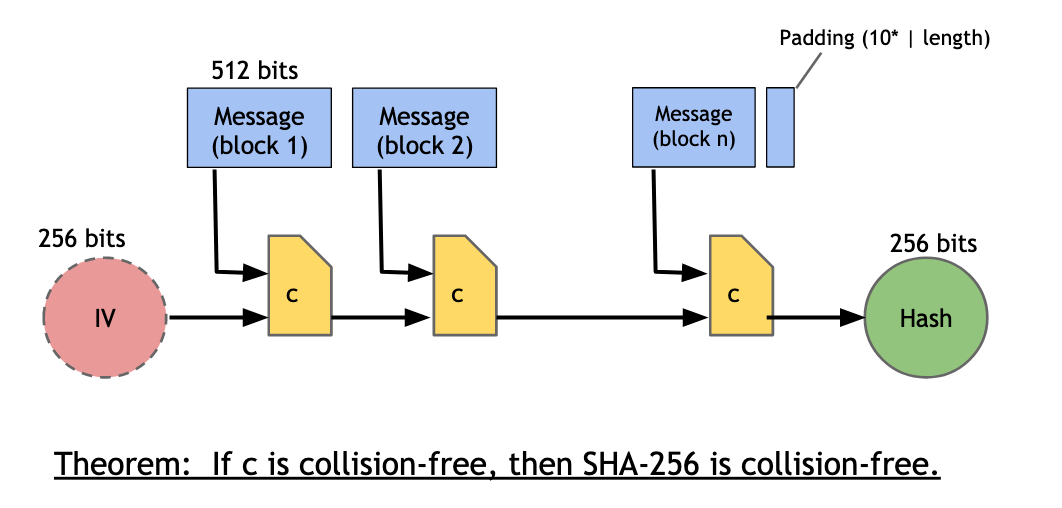
\includegraphics[scale=0.5]{sha}
 
	\begin{itemize}
		\item \textcolor{brown}{SHA-256}: A cryptographic hash function designed by the NSA.
		\item Bitcoin uses $SHA-256^2$ (``SHA-256 squared''), meaning that $H(x)$ actually means $SHA256(SHA256(x))$.

	\end{itemize}

\end{frame}

%%%%%%%%%%%% Slide %%%%%%%%%%%%%%%%%%%%%%%%%%%%%%%%%%%%%%%%%%%%%%%%%%%
\begin{frame}[fragile]
  \frametitle{Generating hash function in Python}
  
	\begin{verbatim}
	import hashlib
	
	hashlib.sha256(string.encode()).hexdigest()
	\end{verbatim}

\end{frame}
%%%%%%%%%%%% Slide %%%%%%%%%%%%%%%%%%%%%%%%%%%%%%%%%%%%%%%%%%%%%%%%%%%
\begin{frame}
  \frametitle{Hash Pointer}
	\begin{itemize}
		\item A pointer to where some info is stored, and
    		\item (cryptographic) hash of the info.
	\end{itemize}

	\pause
	\emph{With a hash pointer, we can}:

	\begin{itemize}
		\item ask to get the info back, and
    		\item verify that it hasn't changed.
	\end{itemize}
\end{frame}
%%%%%%%%%%%% Slide %%%%%%%%%%%%%%%%%%%%%%%%%%%%%%%%%%%%%%%%%%%%%%%%%%%
\begin{frame}
  \frametitle{Key Idea: build data structures with hash pointers}

	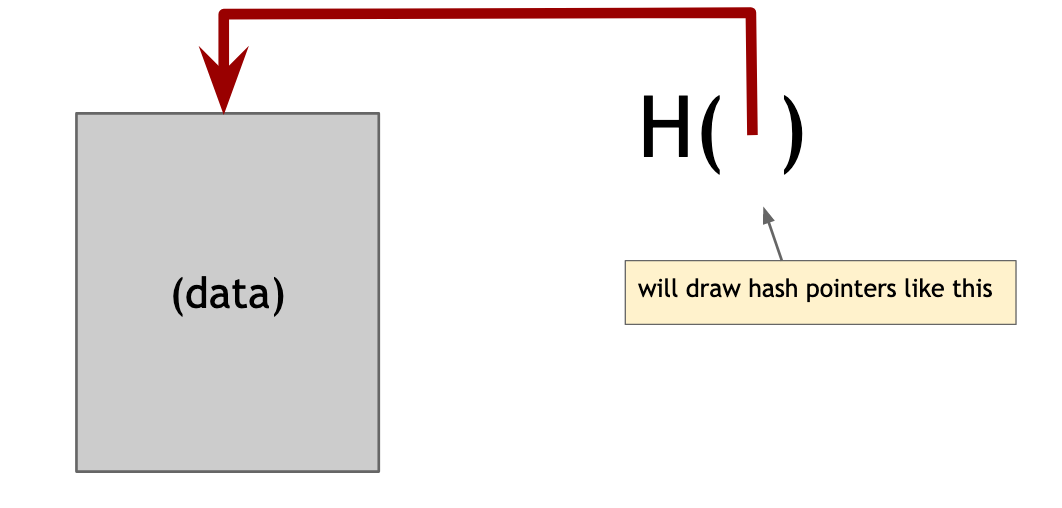
\includegraphics[scale=0.5]{pointer1} 
\end{frame}
%%%%%%%%%%%% Slide %%%%%%%%%%%%%%%%%%%%%%%%%%%%%%%%%%%%%%%%%%%%%%%%%%%
\begin{frame}
  \frametitle{Blockchain}
{\Large{Linked list with hash pointers = ``block chain''}}
	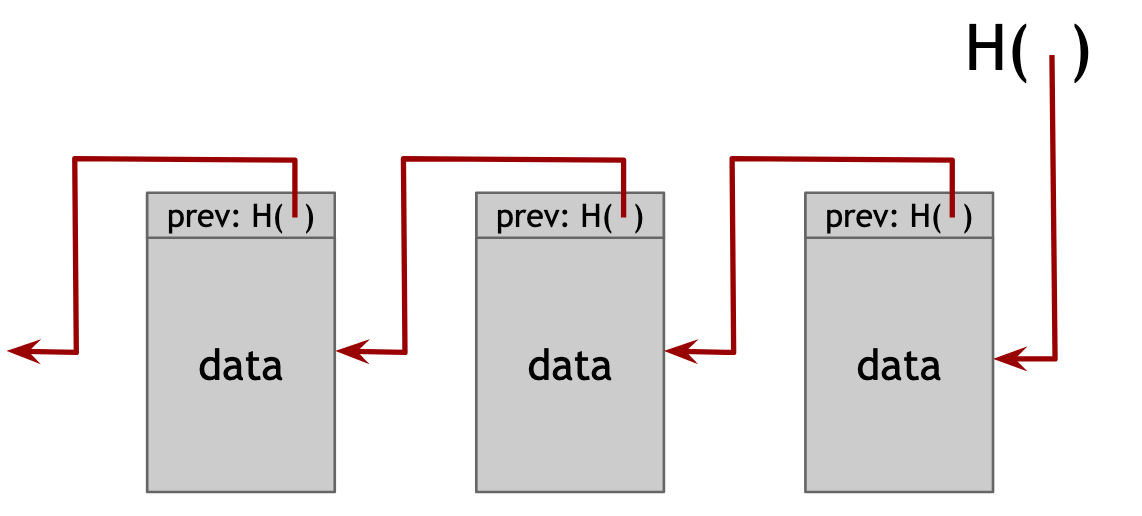
\includegraphics[scale=0.5]{pointer2} 
\end{frame}
%%%%%%%%%%%% Slide %%%%%%%%%%%%%%%%%%%%%%%%%%%%%%%%%%%%%%%%%%%%%%%%%%%
\begin{frame}
  \frametitle{Binary Tree}
{\Large{\textcolor{brown}{Binary tree:} a tree data structure with each node having at most two children.}} \\ 

	\centering 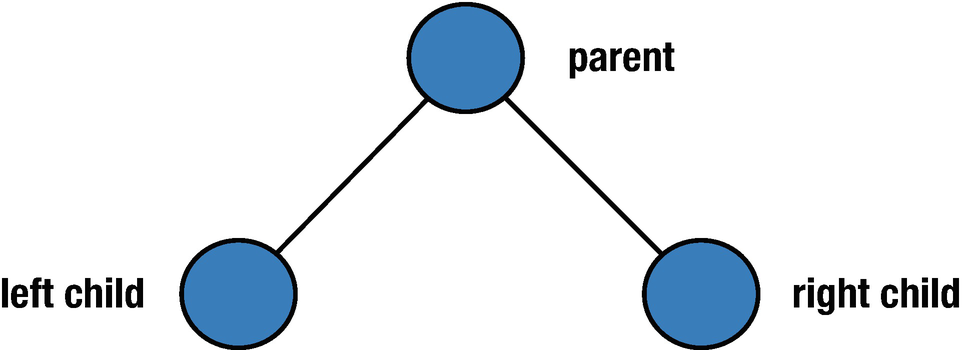
\includegraphics[scale=0.8]{tree} 
\end{frame}
%%%%%%%%%%%% Slide %%%%%%%%%%%%%%%%%%%%%%%%%%%%%%%%%%%%%%%%%%%%%%%%%%%
\begin{frame}
  \frametitle{Merkle Tree}
{\Large{A binary tree with hash pointers}} \\

\centering
	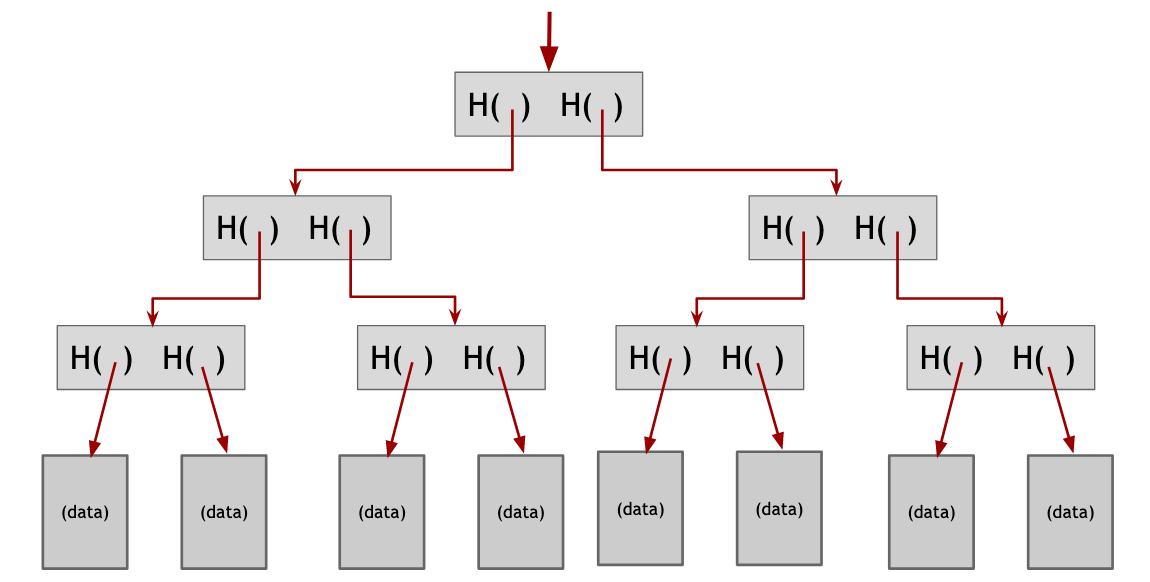
\includegraphics[scale=0.5]{tree1}
\end{frame}
%%%%%%%%%%%% Slide %%%%%%%%%%%%%%%%%%%%%%%%%%%%%%%%%%%%%%%%%%%%%%%%%%%
\begin{frame}
  \frametitle{Advantages of Merkle Trees}
	\begin{itemize}
		\item Just need to remember the root hash.
		\item Can verify membership in $O(log n)$ time/space.
	\end{itemize}
\end{frame}
%%%%%%%%%%%% Slide %%%%%%%%%%%%%%%%%%%%%%%%%%%%%%%%%%%%%%%%%%%%%%%%%%%
\begin{frame}
  \frametitle{Blockchain}
  \centering
	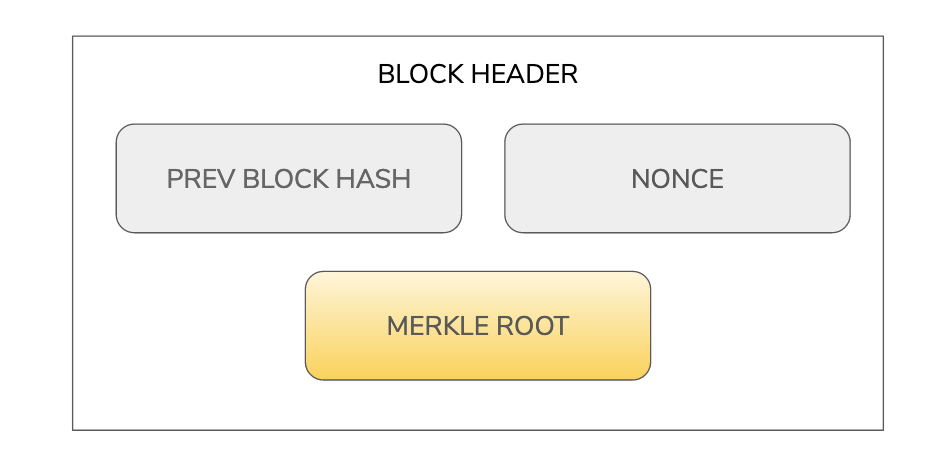
\includegraphics[scale=0.7]{block}
\end{frame}
%%%%%%%%%%%% Slide %%%%%%%%%%%%%%%%%%%%%%%%%%%%%%%%%%%%%%%%%%%%%%%%%%%
\begin{frame}
  \frametitle{Digital Signatures}
	Want:
	\begin{itemize}
		\item Only you can sign, buy anyone can verify.
		\item Signature is tied to a particular document (can't be cut-and-pasted to another doc).

	\end{itemize}
	\pause
	\begin{block}{\textcolor{brown}{Public Key Cryptography:}}  a cryptographic system that allows for secure dissemination of identity and authentication of valid messages.
	\end{block}
\end{frame}
%%%%%%%%%%%% Slide %%%%%%%%%%%%%%%%%%%%%%%%%%%%%%%%%%%%%%%%%%%%%%%%%%%
\begin{frame}
  \frametitle{API for Digital Signatures}

	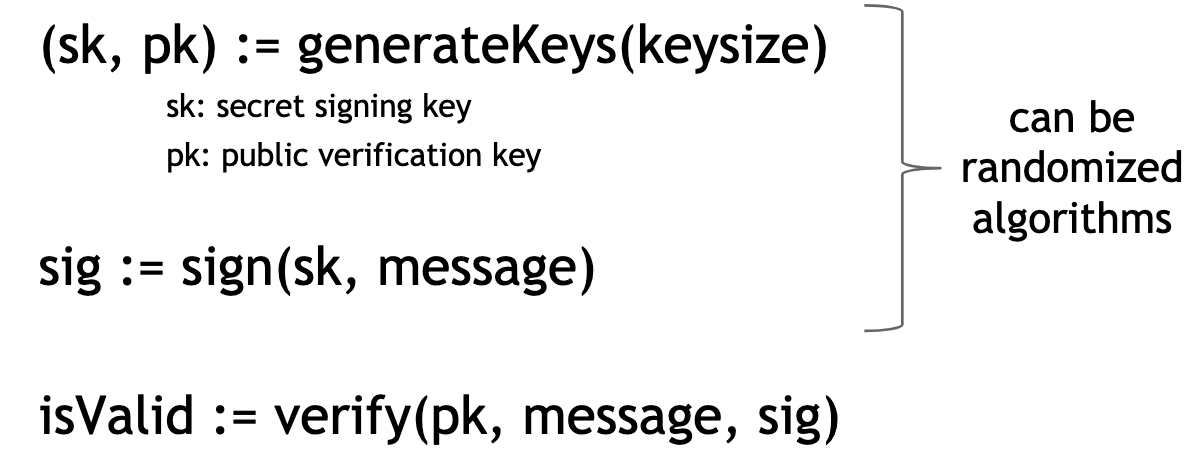
\includegraphics[scale=0.5]{api}
\end{frame}
%%%%%%%%%%%% Slide %%%%%%%%%%%%%%%%%%%%%%%%%%%%%%%%%%%%%%%%%%%%%%%%%%%
\begin{frame}
  \frametitle{ECDSA standard: Elliptic Curve Digital Signature Algorithm}

	\begin{itemize}
		\item The algorithm used by Bitcoin  to generate public keys and verify transactions.
		\item A variant of standard DSA but with elliptic curves.
		\item Good randomness is essential.
	\end{itemize}
\end{frame}
%%%%%%%%%%%% Slide %%%%%%%%%%%%%%%%%%%%%%%%%%%%%%%%%%%%%%%%%%%%%%%%%%%
\begin{frame}
  \frametitle{ECDSA Example}

	Instructor's chicken scratches ... 
\end{frame}
%%%%%%%%%%%% Slide %%%%%%%%%%%%%%%%%%%%%%%%%%%%%%%%%%%%%%%%%%%%%%%%%%%
\begin{frame}[fragile]
  \frametitle{Public Key Generation}

	\begin{verbatim}
Input: public key
Output: corresponding private key

256 bit private key, takes O(sqrt(n)) operations to crack
15 * pow(2,40) hashes per second on the ENTIRE Bitcoin network

pow(2,128) / (15 * pow(2,40)) / 3600 / 24 / 365.25
= 0.6537992112229596e18

650 million billion years

	\end{verbatim}
\end{frame}
%%%%%%%%%%%% Slide %%%%%%%%%%%%%%%%%%%%%%%%%%%%%%%%%%%%%%%%%%%%%%%%%%%
\begin{frame}
  \frametitle{Public Key as Identity}
	Make new identity: 
	\begin{itemize}
		\item Create a new, random key-pair $(sk, pk)$.
		\item You control the identity, because only you know the secret key, $sk$.

	\end{itemize}
\end{frame}
%%%%%%%%%%%% Slide %%%%%%%%%%%%%%%%%%%%%%%%%%%%%%%%%%%%%%%%%%%%%%%%%%%
\begin{frame}
  \frametitle{Decentralized Identity Management}
	\begin{itemize}
		\item Anyone can make a new identity at any time, as many as want.
		\item There is no central point of coordination.
		\item Identities are called \textcolor{brown}{addresses} in Bitcoin.
	\end{itemize}
\end{frame}
%%%%%%%%%%%% Slide %%%%%%%%%%%%%%%%%%%%%%%%%%%%%%%%%%%%%%%%%%%%%%%%%%%
\begin{frame}
  \frametitle{Privacy}
	\begin{itemize}
		\item Addresses not directly connected to real-world identity.
		\item But observer can link together an address's activity over time, make inferences.
		\item Will discuss privacy in Bitcoin in more detail later.
	\end{itemize}
\end{frame}
%%%%%%%%%%%% Slide %%%%%%%%%%%%%%%%%%%%%%%%%%%%%%%%%%%%%%%%%%%%%%%%%%%
\end{document}
